%%%%%%%%%%%%%%%%%%%%%%%%%%%%%%%%%%%%%
% Author: Xiong Yiliang
% Email: wlxiong@gmail.com
% Date: November 23, 2008
% Title: Translation to The Mathematics of Traffic in Networks
%         The Princeton Companion to Mathematics
%%%%%%%%%%%%%%%%%%%%%%%%%%%%%%%%%%%%%
\documentclass[a4paper,12pt, twocolumn]{article}
\usepackage{ctex}
\usepackage{amsmath}
\usepackage{paralist}
\usepackage{geometry}
\usepackage{graphicx}
\usepackage{listings}
\usepackage{mflogo}
\usepackage{psfrag}
\usepackage[small]{caption}

% Page margins
\geometry{textheight=10in, textwidth=7in}

% Redefine names
\renewcommand{\figurename}{图}
\renewcommand{\refname}{参考文献}
\renewcommand{\abstractname}{说明}

% Caption width
%\setlength{\captionwidth}{\linewidth}

\begin{document}

\title{网络中交通流量的数学模型}
\author{熊一梁\\wlxiong@gmail.com\\ 西南交通大学 }
\date{}

\maketitle

\abstract{
这里翻译的是~\emph{The Princeton Companion to Mathematics} 
(Princeton University Press, 2008)~中~Frank Kelly~的短文
\emph{The Mathematics of Traffic in Networks}. 
本文根据作者的~\LaTeX~源文件译出, 与正式出版的文章在个别字句上可能有
细微差别. 由于原文作者是一位数学家, 所以文中的一些术语与交通领域的说法
存在一些差异. 对原文感兴趣的读者可以访问链接: 
\texttt{http://www.statslab.cam.ac.uk/~frank/PAPERS/PRINCETON/}. }

\section{导言}

We are all familiar with congested roads, and 
perhaps also with congestion in other networks,
such as the Internet.  In such networks 
the pattern of traffic flows through different parts 
of the system is the consequence of a subtle and 
complex interaction between different users.
For example, in a road network
we should expect each driver to attempt to choose 
the most convenient route, and this choice 
will depend upon the delays the driver expects to encounter
on different roads; but these delays will in turn 
depend upon the route choices made by others. 
This mutual interdependence makes it difficult to 
predict the effect of changes to the system, for example
the construction of a new road, or  the introduction
of tolls for parts of the system.

我们熟知道路的拥挤甚至其它网络中的阻塞, 比如互联网. 在这类网络中
\footnote{译文中的网络, 系统等词汇一般指城市交通网络或者通信网络, 
读者可以通过上下文来判别. }, 
系统中不同部分的交通流分布是不同用户间微妙复杂作用的结果. 
例如在道路网络中, 我们一般认为每个驾驶者都选取最为便利的路径, 
这种选择取决于驾驶者对不同道路上所经历延误的预期, 但是这些延误
又依赖于其它驾驶者的路径选择. 这种相互依赖的关系使得人们很难去预测
系统变更的影响, 例如修建一条新的道路, 或是在系统的某些地方收取通行费. 

Related issues arise in other large-scale systems,
such as the telephone network or the Internet. 
In such  systems a major practical concern is
the extent to which control can be decentralized.
When you are browsing the web, the rate at which a
webpage is transferred to you across the network is 
controlled by software protocols running on your computer
and on the web server hosting the webpage. This 
decentralised approach to flow control has been
outstandingly successful, as the Internet has
evolved from a small-scale research network to 
today's interconnection of hundreds of millions
of hosts, but is beginning to show signs of strain.
In developing new protocols, 
the challenge is to understand just which aspects of 
decentralized flow control are important if
the network as a whole is to continue to expand
and evolve.

相关的问题也存在于其它的大型系统中, 比如电话网络或者是互联网. 
在这些系统中一个主要的现实问题是分散的控制可以达到怎样的程度.
当你在浏览网页时, 页面通过网络传输到你那的速率是由运行在你的
电脑上和网页所在的服务器上的软件协议控制的. 这种分散控制流量的
方法已经取得了显著的成功. 但是当互联网从一个小型的研究网络演变为
今天的连接着千百万个服务器的大家伙, 互联网出现了超负荷的预兆.
在开发新协议的过程中, 困难的是去认识分散流量控制中哪些方面是关键, 
假如整个网络继续扩张和演变. 

In this article we introduce the reader to some of 
the mathematical models which have been used
to address these issues. The models need to be able to
represent several distinct aspects of the system.
We shall see that the language of graph theory and matrices
is needed to capture the pattern of
connections within the network. The language of calculus
is needed to describe how congestion depends upon traffic 
volumes. And optimization concepts are needed to 
model the way in which self-interested drivers choose
their shortest routes, or decentralized controls in 
communication networks, can result in good system performance.

在本文中我们为读者介绍一些被用来阐述这些问题的数学模型. 
这些模型要能表现系统中数个不同的方面. 我们将会看到图论和矩阵
的知识被用来刻画网络中的连接关系. 微积分的知识被用来描述拥挤
是如何依赖于交通流量的. 并且最优化的概念被用来模拟自私的驾驶者
应该如何选取最短路径或者通信网中的应该采用何种分散控制方式
才能得到良好的系统运行水平. 

\section{网络结构}

Figure~\ref{Fig-pcm0052.1} illustrates a set of  three nodes 
connected by a set of five directed links. 
We might imagine that the nodes represent towns or locations
within a city, and the links 
represent road capacity between different nodes. A two way road
is represented by two links, one in each direction. 
Observe that there are two routes from node $c$  
to node $a$ that a driver could choose: 
the first route, let us call it $ca1$, is the direct 
route, using link $5$; the second route, let us call it $ca2$,
is via node $b$ and uses links $4$ and $2$.  

图~\ref{Fig-pcm0052.1} 所示的是由五条有向边连接的三个节点.
我们可以想象那些节点代表城镇或者城市中的地点, 边代表不同节点间
道路的通行能力. 一条双向道路由两条边来表示, 每个方向个各一条. 
可以看到从节点~$c$~到节点~$a$~有两条路径共驾驶者选择: 第一条
路径, 我们称之为~$ca1$, 通过边~$5$~径直连接; 第二条路径, 我们称之为
~$ca2$, 经过节点~$b$~由边~$4$~和边~$2$~连接.

\begin{figure}[ht]
\centering
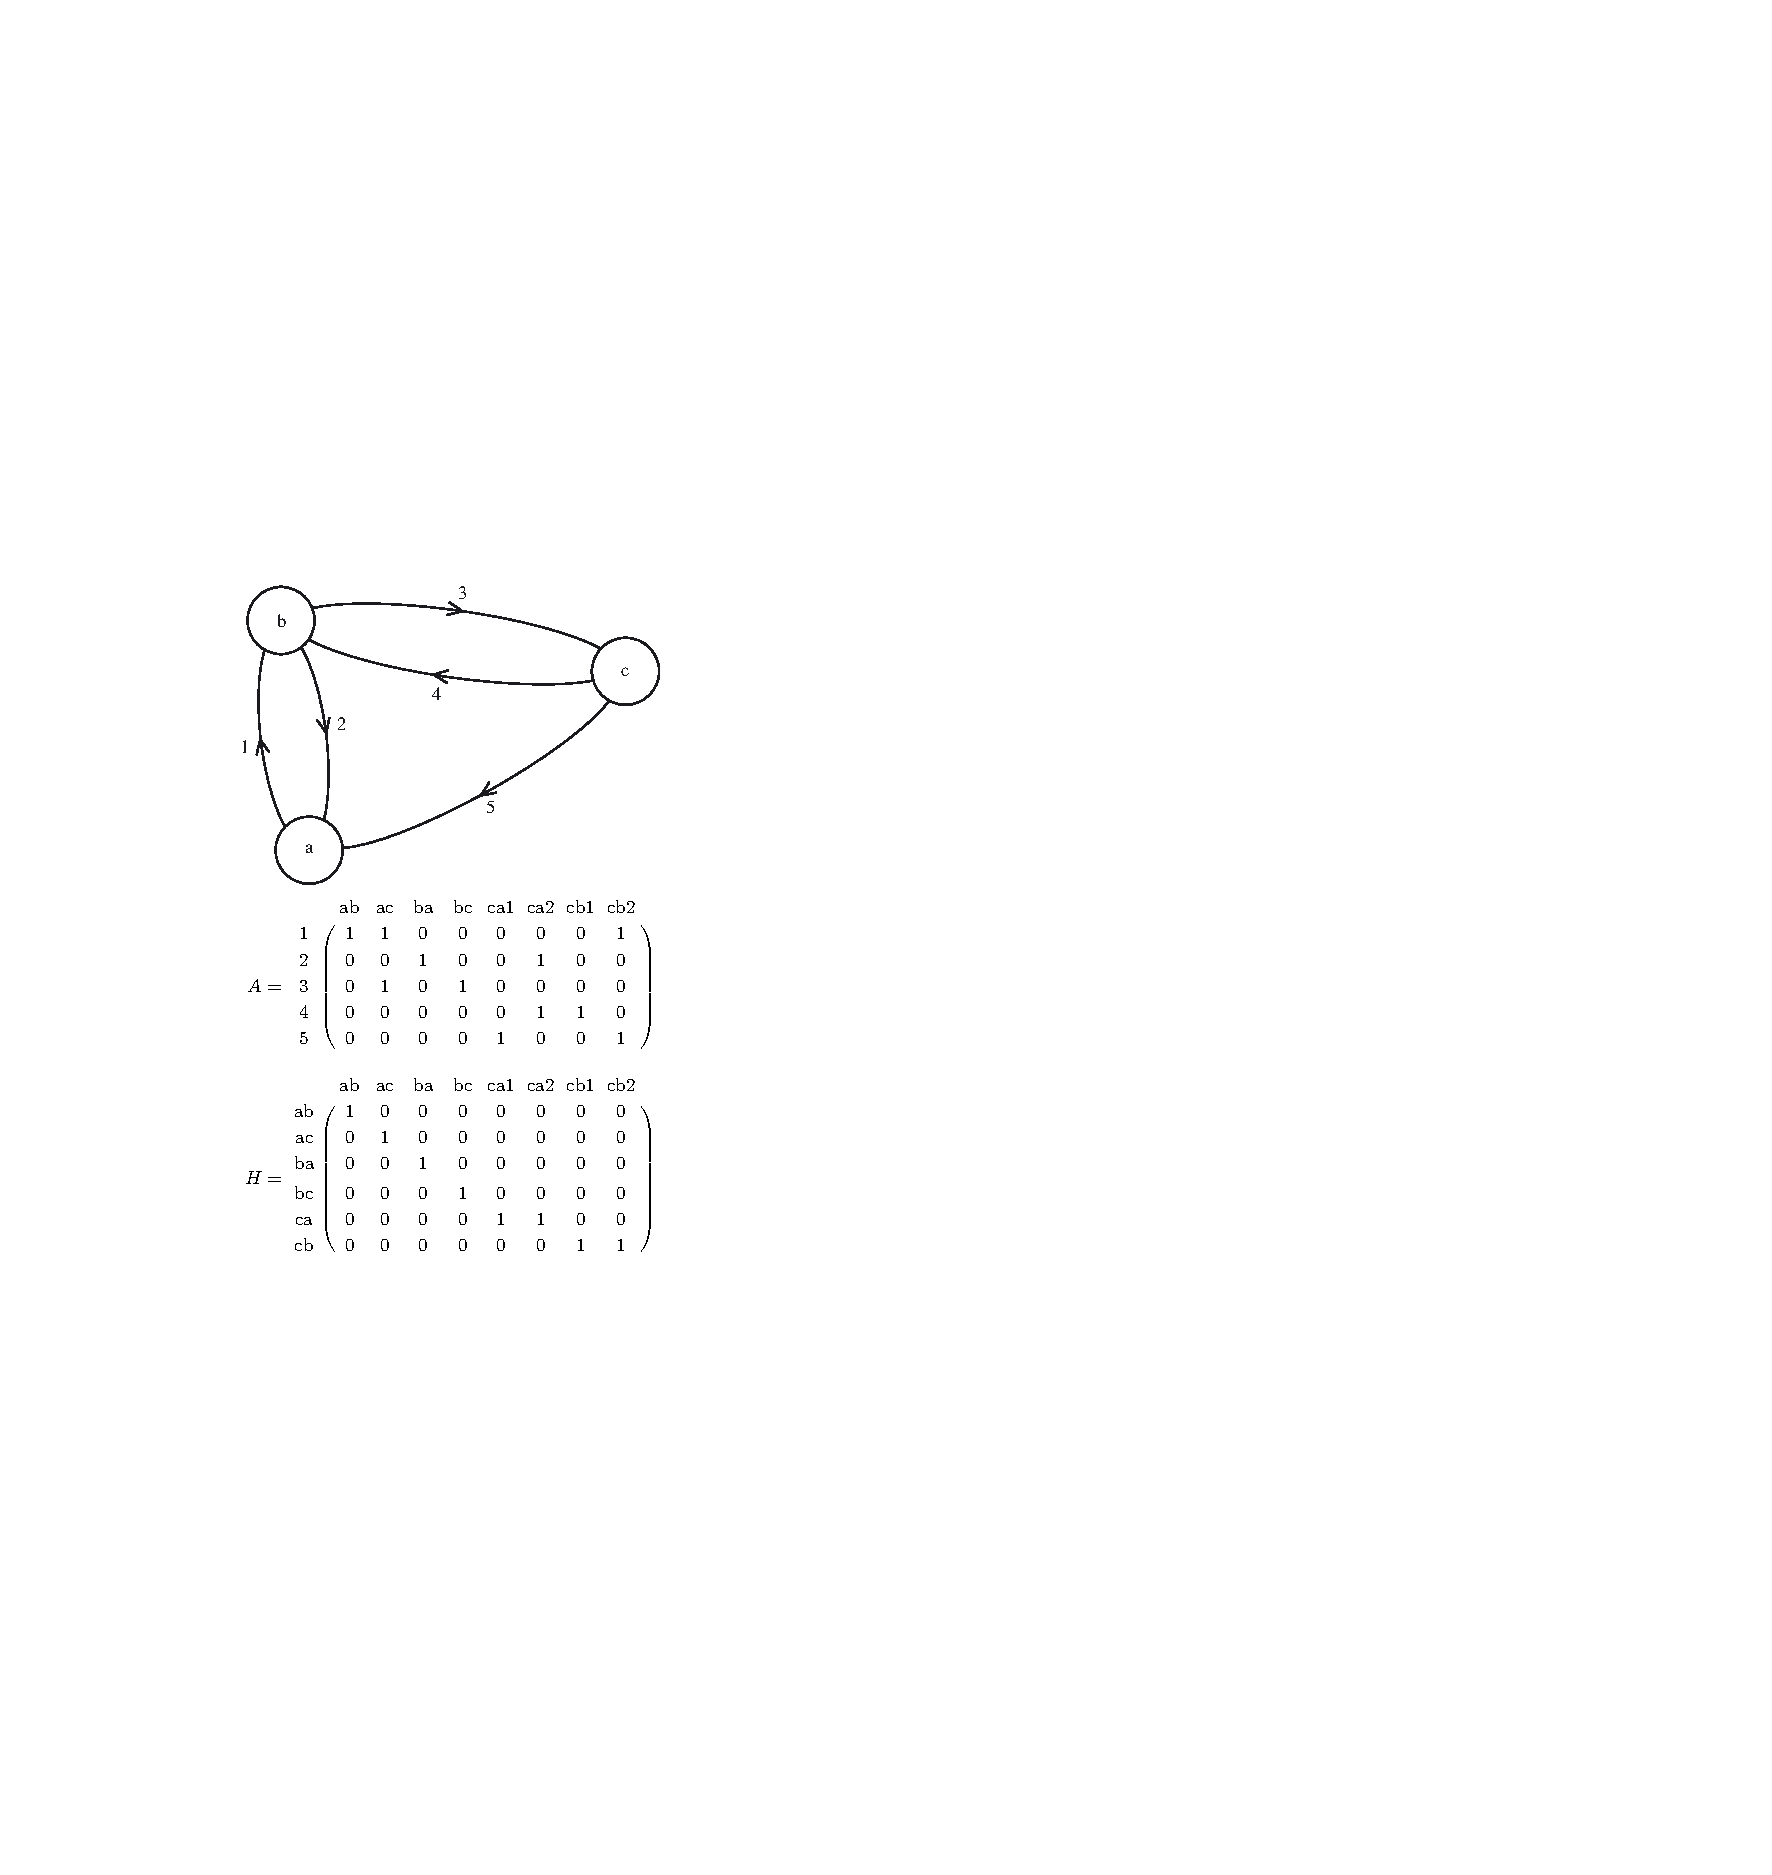
\includegraphics{p1}
\caption{A simple network and its link-route incidence matrix, $A$.
The matrix $H$ represents which routes serve which source-destination pairs.
一个简单网络以及它的路段-路径关联矩阵~$A$. 矩阵~$H$~表示哪些
路径连接着哪些起讫点对.
\label{Fig-pcm0052.1}}
\end{figure}

Let $J$ be the set of directed links, and let $R$ be
the set of possible routes. A way to 
describe the relationship between links and routes is 
with a table, or {\it matrix}, defined as follows.
Set $A_{jr}=1$ if link $j$
lies on route $r$, and set $A_{jr}=0$ otherwise. 
This defines a  matrix $A=(A_{jr}, j\in J, r\in R)$
called the {\it link-route incidence matrix}. Each column
of the matrix corresponds to one of the routes $r$, and each row
to one of the links $j$ of the network. The
column for route $r$ is composed of $0$s and $1$s: the
$1$s tell us which links are on route $r$. 
The $1$s in the row for link $j$ tell us which routes
pass through link $j$. Thus the incidence matrix in
Figure~\ref{Fig-pcm0052.1} shows the two routes, $ca1$ and
$ca2$, between node $c$ and node $a$, and that the first uses 
link $5$ and that the second uses links $4$ and $2$. 
Note that the incidence matrix  does not capture 
the order of the links on the route. 
Also the incidence matrix 
shown does not include all logically possible routes, 
but it could if desired.  And while we have illustrated a
very small network, there is no limit on how many 
nodes and links  could be in the network, or on how
many choices of route each driver might have -- the
incidence matrix would just be bigger. 

令~$J$~为有向边的集合, $R$~为可能路径的集合. 一种描述边和路径间
关系的方法是使用表格, 或\textbf{矩阵}, 定义如下. 令~$A_{jr}=1$~
如果边~$j$~位于路径~$r$~上, 否则令~$A_{jr}=0$. 这就定义了
\textbf{边-路径关联矩阵}~$A=(A_{jr}, j\in J, r\in R)$. 矩阵中的每一列
对应一条路径~$r$, 每一行对应网络中的一条边~$j$. 路径对应的列由
~$0$~和~$1$~组成: $1$表示该边位于路径~$r$~上. 边对应的行中的
~$1$~表示该路径经过边~$j$. 图~\ref{Fig-pcm0052.1}~中的关联矩阵
给出了连接节点~$c$~和节点~$a$~的两条路径~$ca1$~和~$ca2$, 
其中第一条路径使用了边~$5$~而第二条路径使用了边~$4$~和边~$2$. 
需要注意的是关联矩阵没有刻画出路径上各边的顺序. 同样的关联矩阵没有
给出所有理论上可能的路径, 但是如果需要也可以全部给出. 虽然我们仅仅
绘出一个非常小的网络, 实际上网络中节点和边的数目或者是每个驾驶者
能选择的路径数没有限制~---~只是关联矩阵变得更大了. 

In a network, a quantity of interest is the volume of traffic 
along  a particular route or link.
Let $x_r$ be the {\em flow\/} on route $r$, defined as the
number of cars per hour that travel along that route. 
We can list the flows along all the
routes in the network in a single vector $x =(x_r,r \in R)$.
From this vector we can calculate the total flow through a link:
for example, the total flow through link $5$ in Figure~\ref{Fig-pcm0052.1} 
is the sum of flows along routes $ca1$ and $cb2$, since each of
these routes passes through link $5$, and no other routes do.
Recall that a route $r$ passes through link $j$ if
$A_{jr}=1$.  Thus the total
flow through link $j$, added up over all of the routes 
through link $j$, is 
\[
y_j  = \sum_{r \in R} A_{jr} x_r    \quad  j \in J.
\]
Matrix multiplication allows the vector of link flows $y =(y_j,j \in J )$ 
to be expressed succinctly as
\[
y = A x .
\]

在一个网络中, 一个令人感兴趣的量是在特定路径或者边上的交通流量. 
令~$x_{r}$~表示路径~$r$~上的\textbf{流量}, 定义为每小时行驶
在该路径上的车辆数. 我们可以将网络中所有路径上的流量用一个向量
表示~$x =(x_r,r \in R)$. 通过这个向量我们可以计算一条边上的总流量: 
例如, 图~\ref{Fig-pcm0052.1} 中边~$5$~上的总流量为路径~$ca1$~
和~$cb2$~的流量和, 因为这两条路径都经过了边~$5$, 但没有其它的路径
经过. 前面提到过若~$A_{jr}=1$, 则路径~$r$~通过边~$j$. 于是边~$j$~上
的总流量就是对所有通过边~$j$~的路径上的流量进行求和
\[
y_j  = \sum_{r \in R} A_{jr} x_r    \quad  j \in J.
\]
边上的流量向量~$y =(y_j,j \in J )$ ~可以通过矩阵乘法简洁的表示为
\[
y = A x .
\]

We should expect that the level of congestion on a link 
will depend on the total flow on the link, and that this 
will influence the time taken to travel along the link,
which we shall call the {\it delay}.
Figure~\ref{Fig-pcm0052.2} shows a typical form of this
dependence. At small values of the flow $y$ the delay $D(y)$
is just the time taken to travel along an empty road; for 
larger values of $y$ the delay $D(y)$ is larger, and
quite possibly {\it much} larger, owing to
congestion effects.
\footnote{The graph shown in 
Figure~\ref{Fig-pcm0052.2} is single valued. It is quite possible
for the curve representing delay as a function of flow 
to bend back upon itself, so that higher 
delays than shown in the graph correspond to  flows
{\it smaller} than the maximum flow shown there.
You are in this part of the graph when you
experience stop-start driving conditions on a
congested but otherwise 
incident-free highway.  
Part of the aim of traffic management is to keep                         
flows and delays away from this part of the graph,
which we will  not consider further.

We shall assume the graph is
increasing and smooth, which will make more straightforward our
use of calculus later.
Formally, we shall assume that $D(y)$ is
a continuously differentiable
and strictly increasing function of its argument $y$,
as in the graph shown in Figure~\ref{Fig-pcm0052.2}.
}

我们认为边上的拥挤程度取决于边上的总流量, 并且这会影响在该边上
的行驶时间, 我们称之为\textbf{延误}. 图~\ref{Fig-pcm0052.2} 给出了
这种关系的一种典型形式. 在流量~$y$~取较小值的地方, 延误~$D(y)$~
就是驶过一条空旷道路所需的时间; 在流量~$y$~取更大值的地方延误
~$D(y)$~也更大, 由于拥挤效应这种变化可能会非常大. 
\footnote{
图~\ref{Fig-pcm0052.2} 所示函数图像是单值的. 表示延误的曲线很有
可能是一个图像弯曲到自身之上的关于流量的函数, 所以比如图所示
更高的延误值对应着比最大流量小的流量. 当你身处停停走走但无事故的
驾驶状况时, 你所处的交通条件便位于函数图像的这一部分. 交通管理的
部分目的就是避免流量和延误处于函数图像的这一部分, 对这种情形我们
不做进一步考虑. 

我们假设函数图像是递增光滑的, 这让我们接下来更加便捷地运用微积分. 
严格地说, 我们认为~$D(y)$~是关于变量~$y$~的连续可微的递增函数, 
就如图~\ref{Fig-pcm0052.2} 所示的函数图像. }

Let $D_j(y_j)$ be the delay along link $j$ when the flow
through that link is $y_j$; the delay on link $j$ may
depend upon characteristics of link $j$, such as its 
length and width, and hence the necessity for the
subscript $j$ on the function $D_j(y_j)$. 

令~$D_j(y_j)$~表示流量为~$y_{j}$~时边~$j$~上的延误; 边~$j$~上的
延误可能与边~$j$~的特征有关, 比如它的长度和宽度, 所以函数~$D_j(y_j)$~
有必要带上下表~$j$.

\begin{figure}[ht]
\centering

\includegraphics{p2}
\caption{The time taken to travel along a link, $D(y)$,
expressed as function of the total flow $y$ along the link.
As the flow increases, congestion effects cause additional delay.
驶过某一边所需的时间~$D(y)$~作为边上总流量~$y$~的函数. 
当流量增加, 拥挤效应引发了额外的延误. }
\label{Fig-pcm0052.2}
\end{figure}

\subsection{路径选择}

There will in general be 
a variety of possible routes through the
network capable of linking two nodes. For example,
in Figure~\ref{Fig-pcm0052.1} we have seen that the
incidence matrix $A$ records two routes 
between nodes $c$ and $a$. The pair $ca$ is an
example of a source-destination pair: flow
originating  from source $c$ and destined
for node $c$ can use either of $ca1$ or $ca2$,
the two routes which serve this source-destination pair.
We now need another matrix, this one 
to describe the relationship between 
source-destination pairs and routes.
Use $s$ to label a source-destination pair,
and let $S$ be the set of source-destination pairs.
Set $H_{sr}=1$ if the 
source-destination pair $s$ can be served by the route
$r$, and set $H_{sr}=0$ otherwise. This defines a  matrix
$H=(H_{sr},s\in S,r\in R)$;
Figure~\ref{Fig-pcm0052.1} gives an example. 
Observe that
the row labelled $ca$ picks out the two routes, $r = ca1, ca2$, that
serve the source-destination pair $s=ca$. Each
column of $H$ corresponds to a route, 
and contains a single $1$: this identifies the
source-destination pair served by the route. 
For each $r\in R$ let $s(r)$
be the source-destination pair served by route $r$:
for example, in Figure~\ref{Fig-pcm0052.1}, $s(ac)=ac$ 
and $s(ca1)=ca$. 

一般的在网络中有多条路径可以连接两个节点. 例如, 在图~\ref{Fig-pcm0052.1}~
中我们已经看到关联矩阵~$A$~记录了两条连接节点~$c$~和~$a$~的路径. 
点对~$ca$~是个起讫点对的实例: 始于源点~$c$~并且终于汇点~$c$~的
交通流可以使用连接这对起讫点对的路径~$ca1$~或~$ca2$~中的任意一条. 
我们现在需要另一个矩阵来描述起讫点对和路径间的关系. 用~$s$~标记一对
起讫点, 再令~$S$~为起讫点对的集合. 如果起讫点对~$s$~可以由路径~$r$~
连接, 就令~$H_{sr}=1$, 否则令~$H_{sr}=0$. 这就定义了矩阵~$H=(H_{sr},s\in S,r\in R)$.
图~\ref{Fig-pcm0052.1}给出了一个例子. 可以看到标有~$ca$~的一行得到两条
路径~$r = ca1, ca2$~连接起讫点对~$s=ca$. 矩阵~$H$~的每一列对应一条路径, 
该列只有一个~$1$: 这给出了由这一路径连接的起讫点对. 对任意的~$r\in R$~令
~$s(r)$~为由路径~$r$~连接的起讫点对: 例如, 在图~\ref{Fig-pcm0052.1} 中, 
有~$s(ac)=ac$~和~$s(ca1)=ca$. 

From the vector $x =(x_r,r \in R)$
can calculate the total flow from a source to a destination:
for example, the flow from node $c$ to node $a$  in Figure~\ref{Fig-pcm0052.1}
is the sum of flows along routes $ca1$ and $ca2$, since from
the matrix $H$ we see that these are the routes which
serve the source-destination pair $ca$.
More generally, if $f_s$ is  the total flow of traffic added up
over all of the
routes serving source-destination pair $s$, then
\[
f_s  = \sum_{r \in R} H_{sr} x_r    \quad s 
\in S.
\]
Thus the  vector of source-destination flows $f =(f_s,s \in S )$
can be expressed succinctly in matrix form
as
\[
f = H x.
\]

通过向量~$x =(x_r,r \in R)$~可以计算从一个源点到一个汇点的
总流量: 例如, 图~\ref{Fig-pcm0052.1} 中从节点~$c$~到节点
~$a$~的流量是路径~$ca1$~和~$ca2$~上流量的和, 因为从
矩阵~$H$~中, 我们知道这就是连接起讫点对~$ca$~的全部路径. 
更一般的, 若~$f_{s}$~是所有连接点对~$s$~的路径上的流量的和, 
那么
\[
f_s  = \sum_{r \in R} H_{sr} x_r    \quad s 
\in S.
\]
起讫点对的流量向量~$f =(f_s,s \in S )$~可以通过矩阵乘法简洁的
表示为
\[
f = H x.
\]

\section{Wardrop~均衡}

We are now able to approach the central issue: how do the
traffic flows between the various sources and destinations
distribute themselves over the links of the network? 
Each driver
will try to use the quickest route between her source and destination,
but this may make other routes quicker or slower, and cause other
drivers to change. Only when they can't find alternative, quicker routes,
will drivers not have an incentive to change routes.
What does this mean mathematically?

现在我们可以着手处理中心问题: 多个源点和汇点间的交通流量将
如何分布在网络中的边上? 每个驾驶者都尝试使用连接起讫点的
最短路径, 但是这可能导致其它的路径变得更快或者更慢, 并且迫使
其他驾驶者改换路径. 只有当驾驶者无法选择可替代的更快的路径时, 
驾驶者才不会有动机去改变出行路径. 那么在数学上这意味着什么呢? 

Let's first calculate the time taken for a driver to travel along 
route $r$. The column labelled $r$ of the matrix $A$ tells us
which links $j$ are on route $r$. If we add up the
delays on each of these links, we get the time
taken to travel along route $r$ as the expression 
$$\sum_{j\in J } D_j (y_j) A _{jr}. $$ 
Now the driver using route $r$ could have used 
any other route that served the same source-destination pair $s(r)$.
So, for the driver to be content with her choice, we 
require
$$\sum_{j\in J } D_j (y_j) A _{jr}
\leq \sum_{j\in J } D_j (y_j) A _{jr'} $$
for every other route $r'$ that serves the 
same source-destination pair $s(r)$.
%Wardrop noted that the self-interested choices
%of drivers between a particular source and destination would lead 
%journey times on all the routes actually used to be 
%equal, and less than those which would be experienced 
%on an unused route. 

让我们首先来计算驾驶者行驶在路径~$r$~上所需时间. 矩阵~$A$~
上标有~$r$~的一列记录了位于路径~$r$~上的边~$j$. 如果我们
对这些边上的延误进行加和, 我们就得到行驶在路径~$r$~上所需
时间的表达式
$$\sum_{j\in J } D_j (y_j) A _{jr}. $$
既然使用路径~$r$~的驾驶者可以使用其它任何连接起讫点对~$s(r)$~
的路径. 所以, 为了使驾驶者能对自己选择的路径满意, 我们要求
$$\sum_{j\in J } D_j (y_j) A _{jr}
\leq \sum_{j\in J } D_j (y_j) A _{jr'} $$
对每条连接起讫点对~$s(r)$~的路径~$r'$~都满足. 

Define a {\it Wardrop equilibrium} to be a vector $x =(x_r,r\in R)$
of non-negative numbers 
such that for every pair of routes $r, r'$ serving the 
same source-destination pair, 
$$x_r >0\;\,\Rightarrow\;\,\sum_{j\in J} D_j (y_j)A _{jr}
\leq \sum_{j\in J } D_j (y_j) A _{jr'} $$
where $y = Ax$. 
The implication
expresses the defining characteristic of a Wardrop 
equilibrium~\cite{WAR}, 
that if a route $r$ is actively used, then it achieves the
minimum delay over all routes serving its 
source-destination pair $s(r)$. 

定义\textbf{Wardrop 均衡}是一个由非负分量组成的向量~$x =(x_r,r\in R)$~
使得每两个连接相同起讫点对的路径~$r, r'$~都满足
$$x_r >0\;\,\Rightarrow\;\,\sum_{j\in J} D_j (y_j)A _{jr}
\leq \sum_{j\in J } D_j (y_j) A _{jr'} $$
其中~$y = Ax$. Wardrop 均衡的定义意味着如果一个路径~$r$~被使用, 
那么它是所有连接起讫点对~$s(r)$~的路径中延误最小的~\cite{WAR}. 

Does a Wardrop equilibrium exist? It is not at all clear
whether it is possible to find a vector $x$ such that 
all
of the above implications, for the various routes 
through the network, 
are satisfied simultaneously. 
To
answer the question, we shall proceed by addressing a 
seemingly different question: what is the optimum
to the following optimization problem?
$$\openup1\jot \tabskip=0pt plus1fil
\halign to\displaywidth{\tabskip=0pt
\hfil#\quad &$#\hfil$\tabskip=0pt plus1fil&
\llap{#}\tabskip=0pt\cr
Minimize&\displaystyle{\sum\limits_{j\in J} \int\limits_0^{y_j}}
D_j(u)du&\cr
over&x \geq 0, \quad y  &\cr
subject to&H x =f, A x =y. &\cr
}$$
We shall outline why this optimization problem has a solution $(x,y)$,
and why, if $(x,y)$ is a solution, the vector $x$ is a Wardrop equilibrium.

Wardrop 均衡是存在的吗? 我们不能保证能找到一个向量~$x$~
使得对网络中的每条路径上面所有的要求都满足. 
为了回答这个问题, 我们着手一个看似不同的问题: 如下最优化
问题的最优解是? 
$$\openup1\jot \tabskip=0pt plus1fil
\halign to\displaywidth{\tabskip=0pt
\hfil#\quad &$#\hfil$\tabskip=0pt plus1fil&
\llap{#}\tabskip=0pt\cr
Minimize&\displaystyle{\sum\limits_{j\in J} \int\limits_0^{y_j}}
D_j(u)du&\cr
over&x \geq 0, \quad y  &\cr
subject to&H x =f, A x =y. &\cr
}$$
我们将概述为什么这个最优化问题有解~$(x,y)$, 以及为什么
如果~$(x,y)$~是问题的解那么向量就~$x$~达到~Wardrop 均衡.

The optimization problem has some aspects which are
quite natural. An obvious constraint is that the 
flows along each route are non-negative, captured
by the inequality $x \geq 0$. The constraints
$H x =f, A x =y$ just enforce the accounting rules
we have seen earlier, which allow the source-destination
flows $f$ and the link flows $y$ to be calculated from $x$
using the matrices $H$ and $A$ respectively. We view
the source-destination flows $f$ as fixed, to be distributed
over the various routes, but we view the link flows $y$
as varying with $x$, and to be found. 
At a solution to the optimization problem 
$y$ will be non-negative, since $x$ is.  This much
is fairly natural. But the function 
to be minimized is undoubtedly strange. 
The rate of change of the integral 
$$\int\limits_0^{y_j} D_j(u)du$$
with respect to $y_j$ 
is $D_j(y_j)$, by the fundamental theorem
of calculus, and the function to be minimized is the sum of
these integrals over all links. We shall see  
that the
link between a Wardrop equilibrium and the optimization problem 
is a direct consequence of this observation.  

这个最优化问题的某些方面是非常自然的. 一个明显的约束是要求
每条路径上的流量非负, 由通过不等式~$x \geq 0$~刻画. 约束条件
~$H x =f, A x =y$~确保我们前面看到的要求得到满足, 它使起讫点
流量~$f$~和边流量~$y$~可以通过矩阵~$H$~和矩阵~$A$~分别
计算. 我们认为起讫点流量~$f$~是固定的, 它将被分配到各种路径上, 
但是我们认为边流量~$y$~随着~$x$~变化, 是待定的. 当取得最优解时
~$y$~会是非负的, 因为~$x$~是非负的. 这个结果非常自然. 但是
最小化的目标函数无疑是很奇特的. 根据微积分基本定理, 积分函数
$$\int_0^{y_j} D_j(u)du$$
对~$y_{j}$~的变化率是~$D_j(y_j)$, 并且最小化的目标函数是所有
边对应的积分的和. 我们将会看到~Wardrop~均衡和最优化问题的联系
正是这一发现的结果. 

%Firstly, the conditions on the functions $D_j(\cdot), j \in J$, that they
%be continuous and strictly increasing, imply that the function to be
%minimized is a sum of differentiable, concave functions. The feasible region
%$$\{(x,y) : x \geq 0, H x =f, A x =y \}$$
%is a closed and bounded  
%convex set, and this is enough to ensure that there exists a
%solution $(x,y)$ to the optimization problem, and further that a solution
%can be found by the method of {\it Lagrange multipliers}. 
To find a solution to the optimization problem,
we shall use the method of {\it Lagrange
multipliers}. Define the function
\begin{align*}
&L(x ,y ;\lambda ,\mu )   \\
&=\sum_{j\in J}\int_0^{y_j} 
D_j (z)dz+\lambda \cdot (f-H x)-\mu \cdot (y -A x ),
\end{align*}
where $\lambda =(\lambda_s, s \in S), \mu =(\mu_j, j \in J)$,
are vectors of Lagrange multipliers, to be fixed later. 
The idea is that if we make the right choices of Lagrange
multipliers, the minimization of the function $L$
over $x$ and $y$ will find a solution to the original
problem: in particular, the right choices of Lagrange
multipliers will cause  
the constraints $H x =f, A x =y$ to be satisfied automatically.

我们将使用~\textbf{Lagrange~乘数法}来求解这个最优化问题. 
定义函数
\begin{align*}
&L(x ,y ;\lambda ,\mu )   \\
&=\sum_{j\in J}\int_0^{y_j} 
D_j (z)dz+\lambda \cdot (f-H x)-\mu \cdot (y -A x ),
\end{align*}
其中~$\lambda =(\lambda_s, s \in S), \mu =(\mu_j, j \in J)$~是
~Lagrange~乘数向量, 它们是待定的. 思路是如果我们选择合适的
~Lagrange~乘数, 通过~$x$~和~$y$~最小化函数~$L$~将得到
原问题的解: 特别地, 选择合适的~Lagrange~乘数将使约束条件
~$H x =f, A x =y$~自动得到满足.

To minimize the function $L$ we need to differentiate.
First 
$${\frac{\partial L}{\partial y_j}} = D _j (y_j) -\mu_j .$$
Secondly
$${\frac{\partial L}{\partial x_r}} = -\lambda_{s(r)} +\sum_{j\in J}
\mu_j A_{jr};$$
note that the form of the 
matrix $H$ causes the derivative with respect to $x_r$
to pick out exactly one component of $\lambda$, namely $\lambda_{s(r)}$,
and the form of the  matrix $A$ causes the derivative 
to pick out just those components of
$\mu$ that correspond to links on route $r$.  
These derivatives allow us to deduce that
a minimum of $L$ over $x \geq 0, y$ occurs when
$$\mu_j =D_j(y_j) $$
and
\begin{align*}
\lambda_{s(r)}&=\sum_{j\in J} \mu_j A_{jr} \quad \hbox{if $x_r >0$} \\
&\leq\sum_{j\in J} \mu_j A_{jr} \quad \hbox{if $x_r=0$}.
\end{align*}
The equality condition for $\lambda_{s(r)}$
is straightforward:  if $x_r >0$ 
then small variations up or down in $x_r$ should
not decrease the function $L(x ,y ;\lambda ,\mu)$, and hence 
we deduce that the
partial derivative with respect to $x_r$ must be zero.
But if  $x_r =0$ then we can only vary $x_r$ upwards, and so
all we can deduce is that the partial derivative with respect to $x_r$
is non-negative, and from this we deduce the inequality condition
for $\lambda_{s(r)}$.

为了最小化函数~$L$, 我们需要求导. 首先是
$${\frac{\partial L}{\partial y_j}} = D _j (y_j) -\mu_j .$$
再是
$${\frac{\partial L}{\partial x_r}} = -\lambda_{s(r)} +\sum_{j\in J}
\mu_j A_{jr};$$
要注意的是矩阵~$H$~的结构使得对~$x_{r}$~的导数恰好得到
~$\lambda$~的一个分量, 即~$\lambda_{s(r)}$, 而矩阵~$A$~的
结构使得导数恰好得到~$\mu$~中与路径~$r$~上边对应的分量. 
这些导数让我们推导出函数~$L$~关于~$x \geq 0, y$~的最小值
在
$$\mu_j =D_j(y_j) $$
和
\begin{align*}
\lambda_{s(r)}&=\sum_{j\in J} \mu_j A_{jr} \quad \hbox{if $x_r >0$} \\
&\leq\sum_{j\in J} \mu_j A_{jr} \quad \hbox{if $x_r=0$}.
\end{align*}
处得到. 关于~$\lambda_{s(r)}$~的等式是显而易见的: 如果~$x_r > 0$~
那么变量~$x_r$~上下做小范围浮动不会减少函数~$L(x ,y ;\lambda ,\mu)$~
的值, 于是我们推导出关于~$x_{r}$~的偏微分必须等于零. 但如果~$x_r = 0$~
那么我们只能让~$x_{r}$~向上增长, 所以我们推导出关于~$x_{r}$~的偏微分
是非负的, 从这里我们得到了关于~$\lambda_{s(r)}$~的不等式. 

Observe that minimizing the function $L$ corresponds to allowing
the constraints $Hx=f, Ax=y$ to be violated, but charging a
price $\lambda_s$ for any shortfall of the sum $\sum_{r \in R} H_{sr} x_r$
below $f_s$, and a price $\mu_j$ for any excess of the
sum $\sum_{j: j \in J} A_{jr} x_r$ over $y_j$.
From general results on convex optimization it is 
known that it is possible to find Lagrange multipliers $(\lambda, \mu)$
such that a vector $(x,y)$ minimizing $L(x ,y ;\lambda ,\mu)$
satisfies the constraints $Hx=f, Ax=y$,  and that 
the vector $(x,y)$ then solves 
the original optimization problem.

我们发现最小化函数~$L$~允许约束条件~$Hx=f, Ax=y$~
不被满足, 但是对任意的和$\sum_{r \in R} H_{sr} x_r$~小于
~$f_{s}$~增加费用~$\lambda_s$, 还对任意的和
~$\sum_{j: j \in J} A_{jr} x_r$~超出~$y_j$~增加费用~$\mu$. 
从凸优化中的一般结论中可知, 可以找到~Lagrange~乘数
~$(\lambda, \mu)$~使得最小化~$L(x ,y ;\lambda ,\mu)$~的
向量~$(x,y)$~满足约束条件~$Hx=f, Ax=y$, 并且向量~$(x,y)$~
是原最优化问题的解. 

Our solution for the Lagrange multipliers shows that 
they have a simple interpretation: 
$\mu_j$ is the
delay on link $j$, and $\lambda_s$ is the minimum delay over all
routes serving the node pair $s$. The various conditions
established for the multipliers thus show
that an optimum of the objective function
corresponds precisely to a Wardrop equilibrium. 

Lagrange~乘数的解有一个简单的解释: 
$\mu_j$
是边~$j$~上的延误, 而~$\lambda_s$~是连接点对~$s$~的
所路径上的最小延误. 为乘数准备的各种条件表明了目标函数的
最优值恰好对应着~Wardrop~均衡. 

% Since $D_j(z)$ is
%strictly increasing the objective function  is a strictly convex
%function of $\rho$. Hence there is a unique optimum for the flow
%vector $\rho$, although there may be many corresponding values of the
%non-negative vector $x$ satisfying the linear relations.

Thus if traffic in the network distributes itself in
accordance with the self-interested choices of drivers,
the equilibrium flows $(x, y)$ will
solve an optimization problem. This result is 
originally due to Beckmann {\it et al}~\cite{BMW},
and provides a remarkable insight into the equilibrium patterns
achieved in road traffic networks.  The pattern of traffic
resulting from the 
individual decisions of a large number of self-interested drivers 
is as if a central intelligence were 
directing flows to optimize a certain (rather strange)
objective function.

于是如果网络中的流量依照驾驶者自私的路径选择方式来分配, 
平衡流~$(x, y)$~将是一个最优化问题的解. 这个结论最早由
~Beckmann~等人提出~\cite{BMW},  并且给出了道路交通网络中
均衡流的深刻内涵. 通过大量自私的驾驶者的独立选择得到的
交通流分布似乎是受一个集中的智慧体指挥而成为某个目标函数
~(非常奇特)~的最优解. 

The result does {\it not} mean that
average delays in the network will be minimal: and a striking
illustration of this fact is provided by Braess' paradox~\cite{BRA},
which we next describe. 

这个结论并不意味着网络中的平均延误会是最小的: 这一事实的
显著例证就是~Braess~悖论~\cite{BRA}, 我们将在下节阐述它. 

\section{Braess' paradox}

\begin{figure*}[ht]
\centering
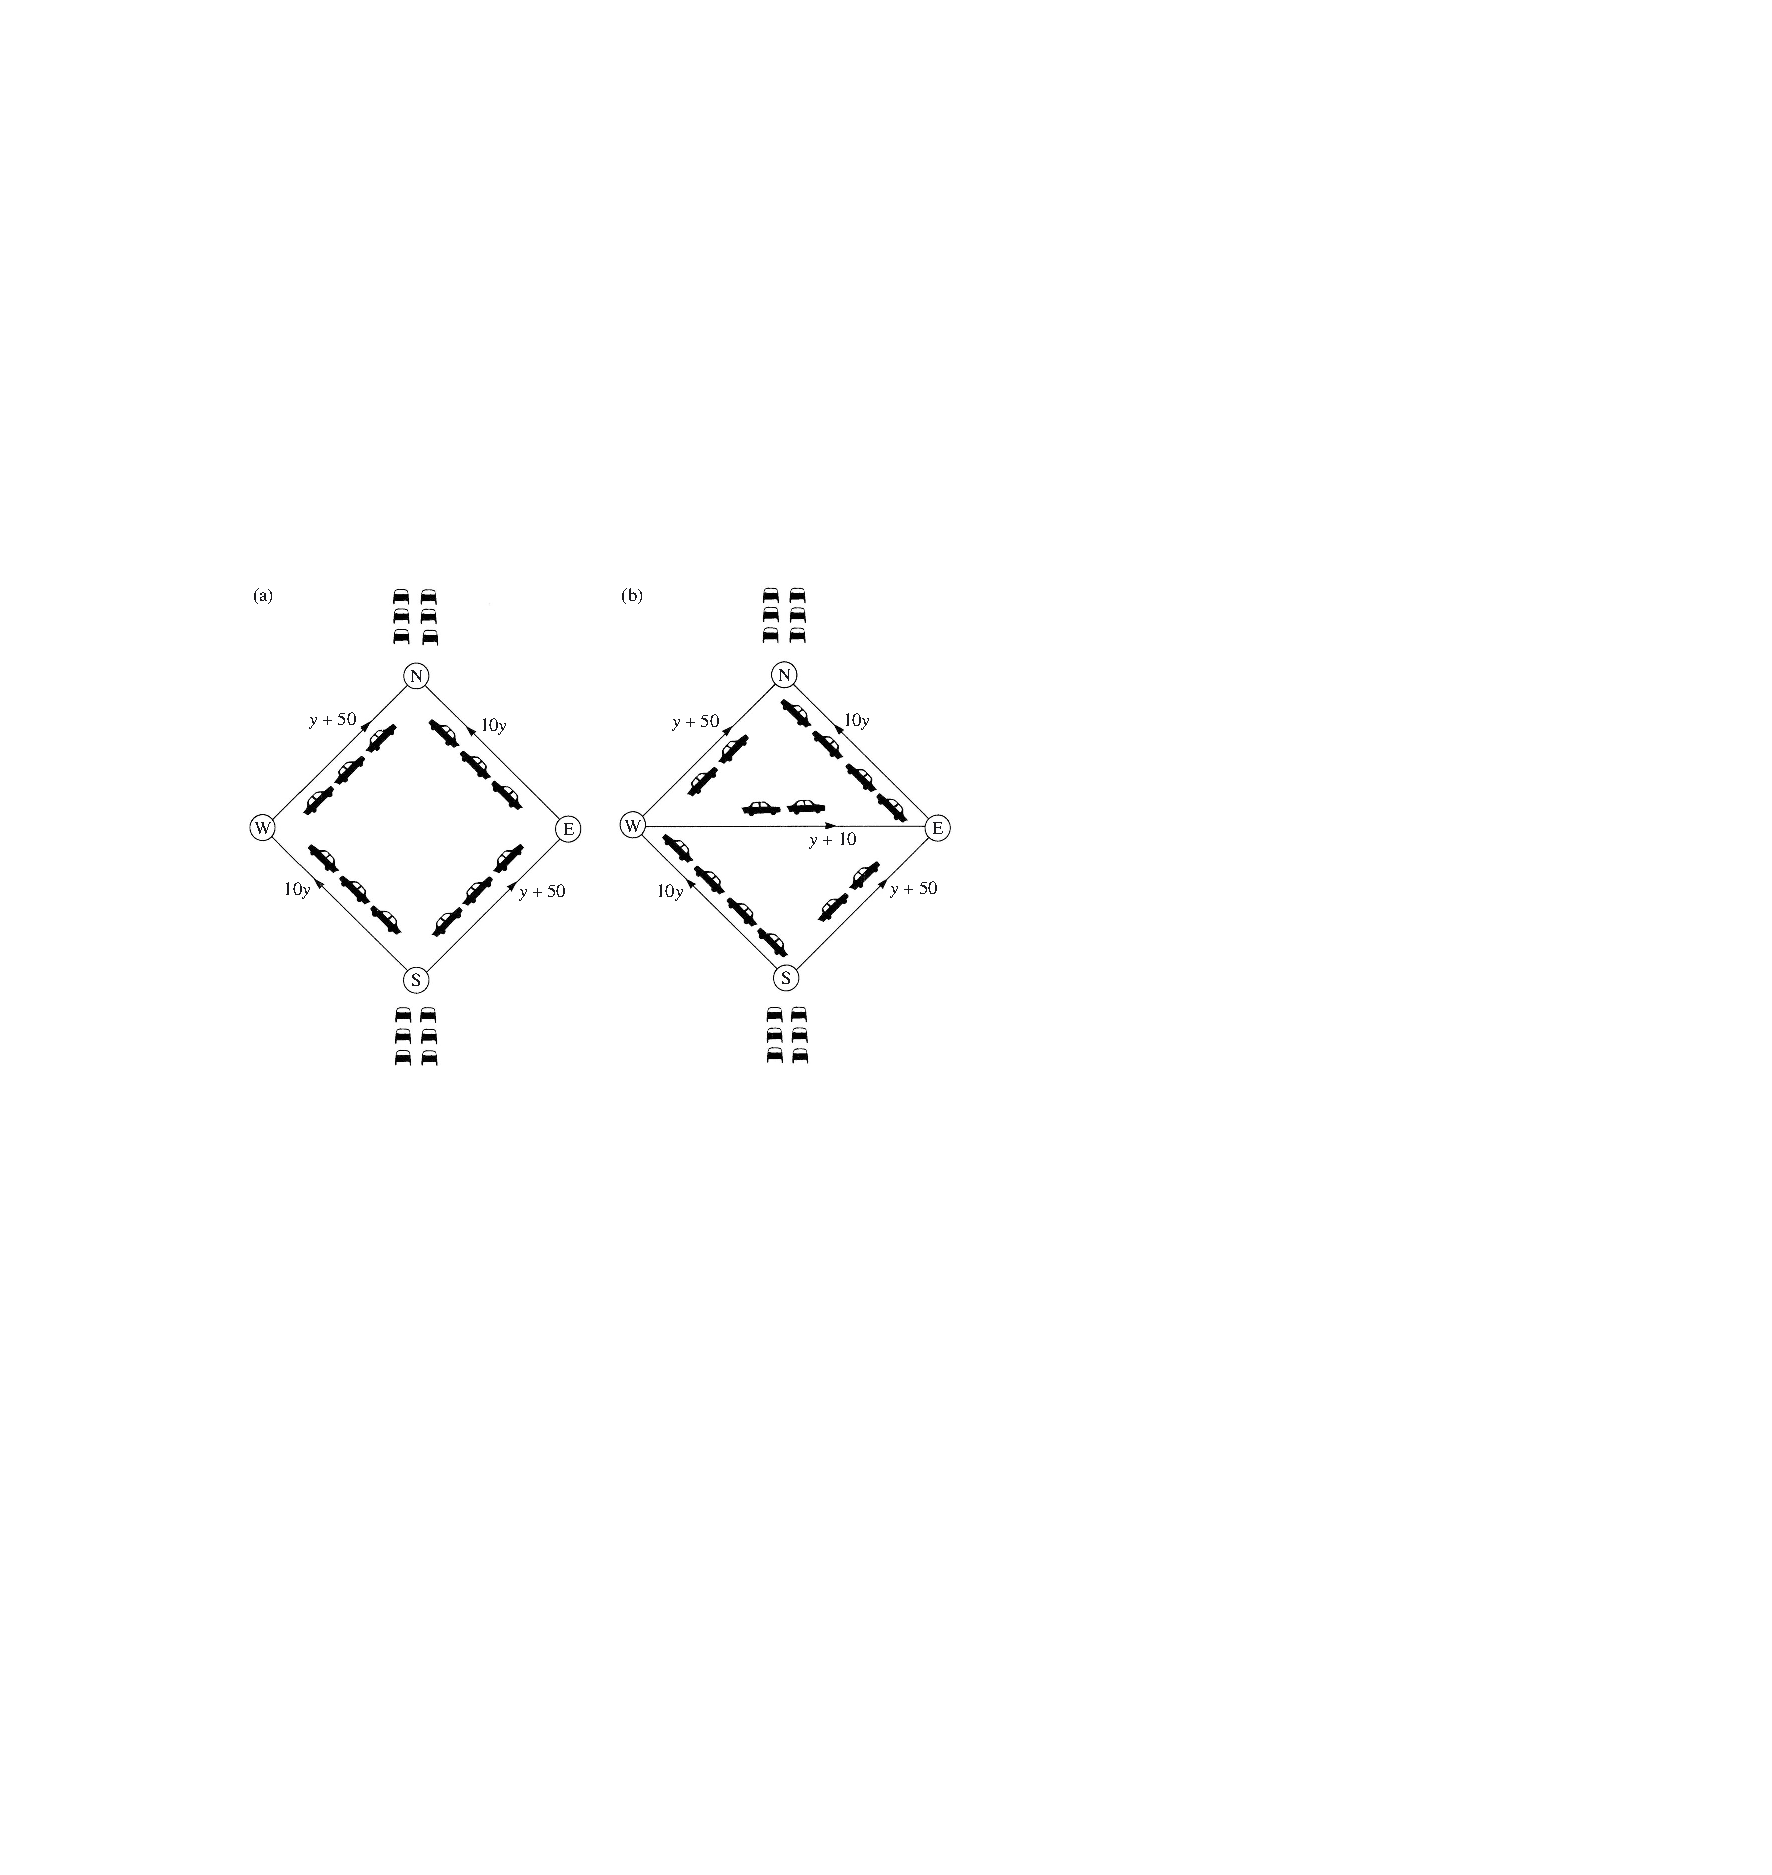
\includegraphics{p3}
\caption{Braess' paradox. The addition of a link causes everyone's
journey time to lengthen. (After~\cite{BRA, COH}.)
Braess~悖论. 增加一条边反而使人们的行程时间加长. 
(参见~\cite{BRA, COH}.)
%(A rough sketch of the figure is in pdf file at
%http://www.statslab.cam.ac.uk/$\sim$frank/PAPERS/pcm.html) 
\label{Fig-pcm0052.3}}
\end{figure*}
 
Consider the network illustrated in 
Figure~\ref{Fig-pcm0052.3}(a). Cars travel 
from node S to node N, via either node W or node E. The total flow is 6, 
and the link delays $D_j(y)$ are given next to links in the
Figure. We might imagine the Figure illustrates 
rush hour as commuters travel from the centre of 
a city in the south, to homes in the north. Commuters 
learn from experience what the delays might be along the eastern
and western routes. The Wardrop equilibrium is shown,
where there is no incentive for any driver to change the route
they use, since both routes incur the same delay,
namely (10 $\times$ 3) + (3 + 50) = 83 units of time.
Now suppose that a new link
is added, between nodes W and E, as shown in 
Figure~\ref{Fig-pcm0052.3}(b). Traffic is
attracted onto the new link, since to begin with it 
offers a shorter journey time from the south to the north.
Eventually, after everyone knows about the new link
and traffic patterns have settled down, there will
be established a new Wardrop equilibrium, shown
in Figure~\ref{Fig-pcm0052.3}(b). In the new equilibrium
there are three routes used, which each incur the same delay,
namely (10 $\times$ 4) + (2 + 50) = 
(10 $\times$ 4) + (2 + 10) + (10 $\times$ 4) = 92. 
Thus in Figure~\ref{Fig-pcm0052.3}(b) 
each car incurs a delay of 92, 
while in Figure~\ref{Fig-pcm0052.3}(a) the delay of
each car had been only 83.
Adding the new link has increased everyone's delay!

考虑如图~\ref{Fig-pcm0052.3}(a)~所示网络. 从节点~S~驶向
节点~N~的车辆经过节点~W~或者节点~E. 总流量为~6, 
边上的延误~$D_{j}(y)$~给出在图中边的旁边. 我们可以想象
图示的是高分小时中通勤者从位于南边的市中心驶回位于
北边的家. 通勤者根据经验知晓了东边的和西边的路径的延误. 
Wardrop~均衡如图所示, 其中没有驾驶者有动机改变他们使用的路径, 
因为两条路径都产生了相同的延误, 即
~$(10 \times 3) + (3 + 50) = 83$~个时间单位. 
现在我们假设加入了一条新的边在节点~W~和节点~E~间, 
如图~\ref{Fig-pcm0052.3}(b)~所示. 交通流被吸引到新的
边上, 因为在一开始它使从南到北的行程时间变得更短. 
最终, 在每个人都知道这条新边后并且交通流分布稳定下来, 
一个新的~Wardrop~均衡建立起来, 如图~\ref{Fig-pcm0052.3}(b)~
所示. 在新的均衡中有三条路径被使用, 各路径产生的延误相同, 即
~$(10 \times 4) + (2 + 50) = (10 \times 4) + (2 + 10) + (10 \times 4) = 92$. 
所以在图~\ref{Fig-pcm0052.3}(b) ~中, 每辆车承当~92~的延误, 
而在图~\ref{Fig-pcm0052.3}(a)~中, 每辆车承当~83~的延误. 
加入的新边增加了人们的延误! 

The explanation for this apparent paradox is as follows.
At a Wardrop equilibrium each driver is 
using a route which, given the choices of others,
gives the minimum delay over the routes 
available between that driver's 
source and destination. But there is no intrinsic reason
why this equilibrium should correspond to particularly low
delays relative to what could be achieved by another
flow pattern.
If all drivers could be
encouraged to depart from their own self-interested choices,
it is quite possible that all might benefit. And in the above example,
if all drivers in the second network could agree to 
avoid the new link, and thus reduce the network
back to the first network, then all would incur lower delays.

对这一表面上的悖论的解释如下. 在~Wardrop~均衡中, 当给定
其他人的路径选择时, 每个驾驶者都选择一条连接起讫点对的
延误最小的路径. 但是并没有固有的理由使这种均衡对应着
某个相比其它交通流分布更低的延误. 如果每个驾驶者被激励
离开他们各自只考虑自身利益的路径, 这很可能使所有的人受益. 
在上面的例子中, 如果在第二个网络中的驾驶者能同意不使用
新的边, 那么网络就退回到第一个网络, 从而产生更低的延误值. 

To explore the point further, note that
the product of the flow $y_j$ and the 
delay $D_j(y_j)$ 
is the  delay incurred at link $j$ per unit time,
aggregated over all the vehicles using link $j$.
Let us try to find the flow pattern which minimizes
the total delay per unit time, summed over the 
entire network.
Consider then the following problem.
$$\openup1\jot \tabskip=0pt plus1fil
\halign to\displaywidth{\tabskip=0pt
\hfil#\quad&$#\hfil$\tabskip=0pt plus1fil&
\llap{#}\tabskip=0pt\cr
Minimize&\displaystyle{ \sum\limits_{j\in J} y_j D_j(y_j)}&\cr
over&x \geq 0, \quad y&\cr
subject to&Hx =f, Ax =y .&\cr}$$
Note that the problem is of the same form as the earlier 
optimization problem, but the function to be minimized 
now measures the total network delay per unit time.
(Recall that the function to be minimized in the first optimization
problem seemed initially to be rather arbitrary, with
its eventual motivation being that its minimization
was achieved by a Wardrop equilibrium.)
Again define the function
\begin{align*}
&L(x ,y ;\lambda ,\mu )  \\
&=\sum_{j\in J}y_j D_j(y_j)+\lambda \cdot
(f-Hx )-\mu \cdot (y -Ax ).
\end{align*}
Again
$${{\frac{\partial L}{\partial x_r}}} = -\lambda_{s(r)} +\sum_{j\in r}\mu_j ,$$
but now
$${{\frac{\partial L}{\partial y_j}} } = D_j(y_j)+ y_jD'_j(y_j)-\mu_j .$$
Hence a minimum of $L$ over $x \geq 0$ and $y$ occurs when
$$\mu_j=D_j(y_j)+ y_jD'_j(y_j)$$
and
\begin{align*}
\lambda_{s(r)}&=\sum_{j\in r}\mu_j\quad \hbox{if $x_r>0$} \\
&\leq\sum_{j\in r}\mu_j\quad \hbox{if $x_r=0$.} \\
\end{align*}

为了进一步探讨这一问题, 需要指出的是流量~$y_{j}$~与延误
~$D_{j}(y_{j})$~的乘积是单位时间内在边~$j$~上的所有车辆
产生的延误的总和. 让我们来试着求解使各个单位时间内整个
网络上的总延误最小的交通流分布. 那么考虑如下问题. 
$$\openup1\jot \tabskip=0pt plus1fil
\halign to\displaywidth{\tabskip=0pt
\hfil#\quad&$#\hfil$\tabskip=0pt plus1fil&
\llap{#}\tabskip=0pt\cr
Minimize&\displaystyle{ \sum\limits_{j\in J} y_j D_j(y_j)}&\cr
over&x \geq 0, \quad y&\cr
subject to&Hx =f, Ax =y .&\cr}$$
这个问题与先前的最优化问题有相同的形式, 但是现在被最小化的
函数是单位时间内整个网络的总延误. (前面提到的第一个最优化
问题中被最小化的函数最初显得很随意, 而最根本的动机是它的
最小化通过~Wardrop~均衡来实现.)
再次定义函数
\begin{align*}
&L(x ,y ;\lambda ,\mu )  \\
&=\sum_{j\in J}y_j D_j(y_j)+\lambda \cdot
(f-Hx )-\mu \cdot (y -Ax ).
\end{align*}
再者
$${{\frac{\partial L}{\partial x_r}}} = -\lambda_{s(r)} +\sum_{j\in r}\mu_j ,$$
但现在有
$${{\frac{\partial L}{\partial y_j}} } = D_j(y_j)+ y_jD'_j(y_j)-\mu_j .$$
于是~$L$~关于~$x \geq 0$ and $y$~的最小值在满足如下条件时
得到
$$\mu_j=D_j(y_j)+ y_jD'_j(y_j)$$
并且
\begin{align*}
\lambda_{s(r)}&=\sum_{j\in r}\mu_j\quad \hbox{if $x_r>0$} \\
&\leq\sum_{j\in r}\mu_j\quad \hbox{if $x_r=0$.} \\
\end{align*}

The Lagrange multipliers now have a more
sophisticated interpretation. Suppose
that, in addition to the delay $D_j(y_j)$, users of link $j$ incur
a traffic dependent toll
$$T_j(y_j)=y_jD'_j(y_j).$$
Then $\mu_j$ is the {\it generalized cost} of using link $j$,
defined as the sum of toll and the delay, and $\lambda_s$ is
the minimum generalized cost over all routes serving the node pair $s$. If
users select routes in an attempt to minimize the sum of their tolls
and their delays, then they will produce a flow pattern which minimizes
total delay in the network.

现在~Lagrange~乘数有了更精细的解释. 假设除了延误~$D_j(y_j)$~
边~$j$~上的用户还被征收一个与交通流相关的通行费
$$T_j(y_j)=y_jD'_j(y_j).$$
那么~$\mu_{j}$~就是使用边~$j$~的\textbf{一般化费用}, 
它被定义为通行费和延误的和, 并且~$\lambda_{s}$~是所有
连接点对~$s$~的路径的一般费用的最小值. 如果用户选择
一条企图最小化他们的通行费和延误的路径, 那么他们会产生
一个使网络总延误最小的交通流分布. 

We have seen that if drivers attempt to minimize their own
delay the resulting equilibrium flows will minimize a certain
objective function defined for the network. However the objective
function is certainly not the total network delay, and thus
there is no guarantee that when capacity is added to a network 
the situation is improved. We have also seen that, with the
imposition of appropriate tolls, it is possible for the
self-interested behaviour of drivers to lead to an equilibrium
pattern of flow that minimizes total delay. A major challenge
for governments and transport planners is to understand how
insights from these and more sophisticated models 
might be used to encourage more efficient 
development and use of road networks~\cite{DfT}.

我们已经看到如果驾驶者企图最小化他们自己的延误, 所得到的
均衡流将使某个根据网络定义的目标函数达到最小值. 然而这个
目标函数显然不是网络的总体延误, 所以这就无法保证何种情况时
扩充网络容量会改善交通状况. 我们也看到, 通过征收适当的通行费
驾驶者的自利行为可能引发一个使总延误最小的均衡分布. 
政府和交通规划者面临的主要困难是领会从这些乃至更精细的模型中
得到的见解可以被怎样的应用以支持更有效的发展和道路网络的应用
~\cite{DfT}. 

\section{互联网中的流量控制}

When a file is requested over the Internet, the source computer
breaks the file into small 
packets of data which 
are then transferred across the network by TCP, the 
transmission control protocol of the Internet.  
The rate at which packets enter the network is
controlled by TCP, 
implemented as software on the computers 
that are the
source and destination of the data.
The general approach is as follows~\cite{JAC}.
When a link within the network becomes overloaded,
one or more packets are lost; loss of a packet is taken as an
indication of congestion, the destination informs the source,
and the source slows down. The TCP then
gradually increases its sending rate until it again receives an
indication of congestion. This cycle of increase and decrease serves
to discover and utilize available capacity, and to share
it between flows. 

在互联网中当一个文件被请求传输时, 起点计算机将文件分作小型的
数据包通过~TCP~协议~(Transmission Control Protocol)~在网络中传送. 
数据包输入到网络中的速率由~TCP~控制, 它在起点和目的地计算机上
以软件形式实现. 一般的方法如~\cite{JAC}~所述. 当网络中的一条边
超负荷了, 一个或者多个数据包丢失; 数据包的丢失被认为是拥堵的信号, 
目的地计算告知起点计算机, 于是起点计算机的传输率下降. 此后~TCP~
逐渐加大其传输率直到再次收到拥堵的信号. 这种增益衰减的循环用来
发现和利用可用的容量, 并且在各流量间分配. 

TCP has been outstandingly successful, 
as the Internet has evolved from a small-scale research network
to today's interconnection of hundreds of millions of endpoints and
links. This in itself is a striking observation.
Each of a large but indeterminate
number of flows is controlled by a feedback loop which
can know only of that flow's experience of congestion.
A flow does not know how many other flows are sharing 
a link on its route, or even how many links are on its route.
The links vary in capacity by many orders of 
magnitude, as do the numbers of flows sharing different links.
That congestion control implemented at the endpoints
can have achieved so much, in such a rapidly growing and 
heterogeneous network, is remarkable.
Why does this algorithm work so well? 

当互联网从一个小规模的研究网络演变为今天连接着千万个节点和边的
网络, TCP~一直以来都非常成功. 这本身就是一个惊人的发现. 大量而又
不确定的流量中的每一个都是由一个仅仅知道其自身经历的拥挤的反馈
回路控制着. 边容量的变化跨越多个数量级, 不同边分担的流量同样如此. 
在一个快速增长并且混杂的网络中, 在端点处执行的拥挤控制策略能有
如此效果是非常了不起的. 为什么这个算法运行得如此好呢? 

In recent years
theoreticians have shed some light on TCP's success,
by interpreting the protocol as a decentralised parallel
algorithm that solves an optimization problem, 
much as we have seen the decentralised choices of drivers in a road
network do. 
We shall outline the argument, beginning with a more
detailed description of TCP.\footnote{Even our detailed description of TCP
is simplified, concerning just the congestion avoidance
part of the protocol, and omitting discussion of timeouts or of
reactions to multiple congestion indication signals received
within a single round-trip time. }

近些年来理论研究者对~TCP~的成功有了一些认识, 他们认为这个协议
是一个求解最优化问题的分散的分布式算法, 和我们看到的道路网络中
驾驶者的分散选择很相似. 我们将概述这个问题, 首先要进一步介绍~TCP. 
\footnote{我们对~TCP~的进一步介绍仍是简略的, 我们只考虑协议中
防止拥挤的部分, 不讨论超时或者在一个往返时间中收到多个拥挤信号时的
对策. }

Packets transferred by TCP across the Internet 
contain sequence numbers, and should
arrive  at the destination in order.  When
a packet is received at the destination, it
is acknowledged: an acknowledgement is a short packet 
sent by the destination back to the source. The source
can deduce from the sequence numbers contained in
acknowledgements if a packet has been lost in transfer. 
The source keeps a copy of
each packet sent until it has been positively acknowledged;
these copies form a {\it sliding window}, and allow packets
lost in transfer to be resent by the source. 

通过~TCP~在互联网中传送的数据包含有序号, 并且必须按照该顺序到达
目的地计算机. 当一个数据包被目的地计算机接受, 将产生一个反馈: 
反馈是从目的地计算机发送到起点计算机的短小的数据包. 起点计算机
可以通过反馈中的序号来判断是否有数据包在传输中被丢失. 起点计算机
保存着每个已发送的数据包的备份, 直到它得到数据已被接收的反馈; 
这些备份形成了一个\textbf{滑动时段}, 在传输过程中丢失的数据包
可以被重新发送. 

The size of the sliding 
window tracks a target {\it congestion window}, stored as 
the variable $\texttt{cwnd}$. It is the rules for
updating $\texttt{cwnd}$ that are critical for TCP's 
sharing of capacity.
In detail, the congestion window 
is incremented by $\texttt{cwnd}^{-1}$ for each positive
acknowledgement, and is halved on detection of a lost 
packet.\footnote{These 
increase and decrease rules may appear rather mysterious,
and indeed it is only recently that many of their macroscopic
consequences have begun to be understood. 
The rules have worked well for more than a decade, but they are now 
beginning to show signs of age, and much current research
is aimed at understanding the full consequences of changing them.}
If the sliding window has fewer packets in it than 
$\texttt{cwnd}$ then the source sends another packet
and thus increases the size of its sliding window by one; and
the sliding window naturally decreases in size by one upon a 
positive acknowledgement. Thus 
the size of the sliding window maintained by the source effectively 
tracks the target value $\texttt{cwnd}$. 

滑动时段的大小跟随着一个目标\textbf{拥挤时段}, 它被保存为变量
~$\texttt{cwnd}$. 更新~$\texttt{cwnd}$~的准则是~TCP~容量分配的
关键. 仔细的说, 每个正反馈会使拥挤时段增长~$\texttt{cwnd}^{-1}$, 
出现一个数据包的丢失将使拥挤时段减半.
\footnote{
这些增益和衰减的规则显得不可思议, 实际上直到最近他们的许多宏观
影响才开始被认识到. 这些规则十多年来都运转良好, 但是他们现在开始
显示出陈旧的迹象, 当前的许多研究着眼于认识改变这些规则所造成的
全部影响. }
如果滑动时段中存在的数据包少于~$\texttt{cwnd}$, 那么起点计算机
将多发送一个数据包, 滑动时段增加一; 一个正反馈使滑动时段减少一. 
因此由起点计算机来保持的滑动时段大小跟随着目标值~$\texttt{cwnd}$. 

The expected change in the 
congestion window \texttt{cwnd} per update step is thus approximately
\[
  \texttt{cwnd}^{-1} \ (1-p)  -  \frac{1}{2} \texttt{cwnd}  \ p
 \]
where $p$ is the probability a packet is lost.
The expected change will be positive for small values of
$\texttt{cwnd}$, but will become negative if $\texttt{cwnd}$
is big enough. We might therefore expect an equilibrium
for $\texttt{cwnd}$ to arise when the expression is zero,
that is when
\[
  \texttt{cwnd} = \sqrt{\frac{2(1-p)}{p} }.
\]

每次更新拥挤时段改变的数学期望大概是
\[
  \texttt{cwnd}^{-1} \ (1-p)  -  \frac{1}{2} \texttt{cwnd}  \ p
 \]
 其中~$p$~为一个数据包丢失的概率. 对于较小的~$\texttt{cwnd}$~值, 
 变化的均值为正, 但是如果~$\texttt{cwnd}$~足够大, 它将变成负的. 
 所以我们猜测当上式为零时~$\texttt{cwnd}$~达到均衡, 即有
 \[
  \texttt{cwnd} = \sqrt{\frac{2(1-p)}{p} }.
\]

Next we describe how this calculation can be extended
to a network. Suppose the network comprises a set of nodes
connected by directed links, as for example illustrated in
Figure~\ref{Fig-pcm0052.1}. As earlier, let $J$ be the 
set of directed links, let $R$ be the set of routes,
and use the link-route incidence 
matrix $A = (A_{jr}, j \in J,  r \in R)$.
Let $x_r = \texttt{cwnd}_r / T_r$, where $\texttt{cwnd}_r$ is
the congestion window for the connection over route $r$ and $T_r$
is the round-trip time between the
source and the destination for route $r$. Since it takes a time
$T_r$ to tranfer $\texttt{cwnd}_r$ packets,
we can interpret $x_r$ as the rate
at which packets are transferred over route $r$. 
Again define $y =Ax$, so that the $y_j$ is the 
total flow through link $j$, obtained by summing $x_r$
over each route $r$ that passes through link $j$. 

下面我们讲述如何将这些计算推广到网络上. 假设网络由一些通过
有向边连接的节点组成, 例如图~\ref{Fig-pcm0052.1}~所示网络. 
如前面一样, 令~$J$~是有向边集合, $R$~是路径集合, 并且使用
边-路径关联矩阵~$A = (A_{jr}, j \in J,  r \in R)$. 
令~$x_r = \texttt{cwnd}_r / T_r$, 其中~$\texttt{cwnd}_r$~是
路径~$r$~上连接的拥挤时段, $T_{r}$~是往返路径~$r$~的
起讫点所需的时间. 由于传送~$\texttt{cwnd}_r$~个数据包需耗时
~$T_{r}$, 我们可以把~$x_{r}$~解释为路径~$x_{r}$~上数据包的
传输率. 再定义~$y = Ax$, 于是~$y_{j}$~为边~$j$~上的总流量, 
通过对每条经过边~$j$~的路径的流量~$x_{r}$~进行求和得到. 

Let $p_j$ be the proportion
of packets that are dropped at link $j$. We expect $p_j$ to
be related to $y_j$, the total flow through link $j$, as follows.
If $y_j$ is less than the capacity $C_j$ of link $j$, then
$p_j$ will be zero -- there will be no dropped packets
at link $j$ if the link is not full. And
if $p_j>0$ then $y_j=C_j$ -- if packets are dropped then
the link is full. 
We assume the proportions of packets dropped at links 
are small: the probability a packet is lost on route $r$
is then approximately
\[
p_r = \sum_{j\in r} p_j.
\]
And since $x_r = \texttt{cwnd}_r / T_r$, our earlier
calculation now gives us that
\[
  x_r = \frac{1}{T_r} \sqrt{\frac{2(1-p_r)}{p_r }}.
\]

令~$p_{j}$~为边~$j$~上的丢包比例. 我们认为~$p_{j}$~与流经
边~$j$~的总流量~$y_{j}$~相关, 如下所示. 若~$y_{j}$~小于
边~$j$~的容量~$C_{j}$, 那么~$p_{j}$~为零~---~边~$j$~上没有
数据包丢失, 如果该边不饱和的话. 若~$p_j>0$~那么~$y_j=C_j$~---~
若有数据包丢失则边是饱和的. 我们假设边上数据包丢失的比例很低: 
一个数据包在路径~$r$~上丢失的概率约为
\[
p_r = \sum_{j\in r} p_j.
\]
有因为~$x_r = \texttt{cwnd}_r / T_r$, 前面的计算现在给出
\[
  x_r = \frac{1}{T_r} \sqrt{\frac{2(1-p_r)}{p_r }}.
\]

Is it possible to choose the rates $x = (x_r, r \in R)$ 
and the drop probabilities $p = (p_j, j \in J)$ in a 
consistent fashion, so that that 
the last two equations are satisfied
and either $p_j$ is zero
or $y_j = C_j$ for each $j \in J$?
The remarkable observation is that 
such a choice corresponds precisely to the solution
of the following optimization problem~\cite{KEL, LPD}.
$$\openup1\jot \tabskip=0pt plus1fil
\halign to\displaywidth{\tabskip=0pt
\hfil#\quad &$#\hfil$\tabskip=0pt plus1fil&
\llap{#}\tabskip=0pt\cr
Maximize&
\displaystyle{\sum_{r\in R} \frac{\sqrt{2} }{T_r} 
\arctan \left( \frac{x_r T_r}{\sqrt{2} } \right)}
&\cr
over&x \geq 0  &\cr
subject to& A x \leq C . &\cr
}$$

是否可以选取相符的流量~$x = (x_r, r \in R)$~和丢包率
~$p = (p_j, j \in J)$~使得最后的两个等式得到满足, 且对任意的
~$j \in J$~要么~$p_j$~为零, 要么~$y_j = C_j$? 重要的发现是
这样的选择恰好对应如下最优化问题的解~\cite{KEL, LPD}. 
$$\openup1\jot \tabskip=0pt plus1fil
\halign to\displaywidth{\tabskip=0pt
\hfil#\quad &$#\hfil$\tabskip=0pt plus1fil&
\llap{#}\tabskip=0pt\cr
Maximize&
\displaystyle{\sum_{r\in R} \frac{\sqrt{2} }{T_r} 
\arctan \left( \frac{x_r T_r}{\sqrt{2} } \right)}
&\cr
over&x \geq 0  &\cr
subject to& A x \leq C . &\cr
}$$

Some aspects of this optimization problem 
are as we might expect: in particular, 
the inequality $A x \leq C$
simply adds up the flows through link $j$ and requires
that the sum not exceed the capacity $C_j$ of link $j$,
for each link $j \in J$.  But, as before, the function
being minimized is undoubtedly strange.  The arctan
function, illustrated in Figure~\ref{Fig-pcm0052.4}, 
is the inverse function to the trigonometric 
function tan, and can also be defined as
$$
\arctan(x) = \int_0^{x}\frac{1}{1+u^2} du. 
$$
From this form, we see that its derivative with respect to $x$ is $1/(1+x^2)$.

对这个最优化问题我们容易想到的一些方面是: 特别是不等式
~$A x \leq C$~就是将通过边~$j$~的流量加起来, 并要求对任意的
~$j \in J$~这个和不超过边~$j$~的容量~$C_{j}$. 但是, 就像前面
一样, 需要最小化的函数的确奇特. 如图~\ref{Fig-pcm0052.4}~
所示的函数~$arctan$~是三角函数~$tan$~的反函数, 它可以被定义为
$$
\arctan(x) = \int_0^{x}\frac{1}{1+u^2} du. 
$$
通过这一形式, 我们发现它对~$x$~的导数是~$1/(1+x^2)$.

\begin{figure}[ht]
\centering

\includegraphics{p4}
\caption{The arctan function.  The Internet's
transmission control protocol, TCP, implicitly maximizes
a sum of utilities over all the connections present in
a network: this function shows the shape
of the utility function for a single connection.
The horizontal axis is proportional to 
the rate of the connection, and  the vertical
axis is proportional to the usefulness of that rate.  Both axes are
scaled in terms of the round-trip time of the connection. 
arctan~函数. 互联网的传输控制协议~(TCP)~暗含着对网络中所有
连接的效率之和的最大化: 这个函数展现了单个连接的效率函数的
形状, 并且纵坐标正比于流量的效用. 两个坐标轴都以连接的往返
时间为标度. 
\label{Fig-pcm0052.4}}
\end{figure}

We next sketch the relationship between the 
optimization problem and the equilibrium rates and 
drop probabilities.  Define the function
\begin{align*}
&L(x,z  ; \mu )  \\
&=\sum_{r\in R} \frac{\sqrt{2} }{T_r}    
\arctan \left( \frac{x_r T_r}{\sqrt{2} } \right)
+\mu \cdot (C -Ax-z ),
\end{align*}
where $\mu = (\mu_j, j \in J)$ is a vector of Lagrange
multipliers, and $z = C- Ax$ is a vector of {\it slack variables},
measuring the spare capacity on each of the links $j \in J$ of
the network. Then, using the derviative of the arctan function,  
$${{\frac{\partial L}{\partial x_r}}} = 
 \left( 1 +
\frac{x_r^2T_r^2}{2} \right)^{-1} 
 -\sum_{j\in J}\mu_j A_{jr}
$$
and
$${{\frac{\partial L}{\partial z_j}}} = -\mu_j. $$
We look for a maximum of $L$ over $x, z \geq 0$;
it turns out that this maximum
is, under the identification $\mu_j = p_j$,
precisely the collection $(x_r, r \in R), (p_j, j \in J)$
sought for rates and drop probabilities. For example,
setting to zero the partial derivative with respect to $x_r$
gives precisely the desired equation for $x_r$.

我们下面简述最优化问题和均衡流量以及丢包率间的关系. 
定义函数
\begin{align*}
&L(x,z  ; \mu )  \\
&=\sum_{r\in R} \frac{\sqrt{2} }{T_r}    
\arctan \left( \frac{x_r T_r}{\sqrt{2} } \right)
+\mu \cdot (C -Ax-z ),
\end{align*}
其中~$\mu = (\mu_j, j \in J)$~为~Lagrange~乘数向量, 
$z = C- Ax$~为\textbf{松驰变量}向量, 它度量了网络中
每条边~$j \in J$~上的剩余容量. 那么, 使用~$arctan$~
函数的导数, 
$${{\frac{\partial L}{\partial x_r}}} = 
 \left( 1 +
\frac{x_r^2T_r^2}{2} \right)^{-1} 
 -\sum_{j\in J}\mu_j A_{jr}
$$
且
$${{\frac{\partial L}{\partial z_j}}} = -\mu_j. $$
我们寻求函数~$L$~在~$x, z \geq 0$~上的最大值; 在保证
~$\mu_j = p_j$~的情况下这个最大值恰是我们要寻求的
流量和丢包率~$(x_r, r \in R), (p_j, j \in J)$. 例如, 令对~$x_{r}$~
的偏导数为零就是关于~$x_{r}$~的要求的方程. 

In summary, the Lagrange multiplier $\mu_j$ arising from
the optimization problem  is precisely the 
proportion of packets dropped $p_j$, for each link $j \in J$, 
much as the Lagrange multipliers arising earlier
were precisely the delays on 
links of a road traffic network. And the equilibrium
reached by the interaction of many competing TCPs,
each implemented only on the source and destination computers, 
is effectively maximizing an objective function for the
entire network. The objective function has a surprising  
interpretation: it is as if the usefulness of
the flow rate $x_r$ to the source-destination pair 
served by this route is given by a {\it utility function}
\[
 \frac{\sqrt{2} }{T_r}
\arctan \left( \frac{x_r T_r}{\sqrt{2} } \right),
\]
and the network is attempting to maximize the sum of these
utility functions across all source-destination pairs, 
subject to the link capacity constraints.

简而言之, 最优化问题中的~Lagrange~乘数~$\mu_{j}$~恰巧是
每条边~$j \in J$~上的丢包率~$p_{j}$, 这与前面道路交通网络
上边的延误相似. 并且由大量仅在起点和目的地计算机上实现的
相互竞争的~TCP~达到的均衡有效的最大化了整个网络的目标函数. 
这个目标函数有一个令人惊奇的解释: 流量~$x_{r}$~对该边
连接的起讫点对的有效性由如下效用函数给出
\[
 \frac{\sqrt{2} }{T_r}
\arctan \left( \frac{x_r T_r}{\sqrt{2} } \right),
\]
并且网络企图在边容量的约束下, 最大化所有起讫点对的效用函数之和. 

The arctan function, illustrated in Figure~\ref{Fig-pcm0052.4},
is {\it convex}.  Thus, if two or more connections share an
overloaded link then the rates the connections achieve 
will be approximately 
equal, since otherwise the total utility could be increased
by reducing a little the largest rate and increasing a 
little the smallest rate. There is thus a tendency for TCP to 
share resources more or less equitably. 
This is in contrast with resource control
mechanisms in traditional telephony networks
where,  if the network is overloaded, some calls
are blocked in order
that calls accepted are unaffected by the overload.

如图~\ref{Fig-pcm0052.4}~所示的~arctan~函数是\textbf{凸函数}. 
所以如果一个或者多个连接分配在一个超负荷的边上, 那么各连接
达到的流量大致是相等的, 因为如果不这样可以通过减小一些最大的
流量而增加一些最小的流量来加大总效用. TCP~有差不多均匀分配
资源的趋势. 这不同于传统的电话网络的机制, 如果电话网络超负荷, 
为了使接受的通话不被超负荷影响, 一些通话会被阻止. 

\section{Conclusion}

The behaviour of large scale systems has been of great interest to
mathematicians for over a century, with many examples coming from
physics. For example, 
the behaviour of a gas can be described at the microscopic
level in terms of the position and velocity of each molecule. At this
level of detail a
molecule's velocity appears as a random process, as 
the molecule bounces around off other molecules and the
walls of the 
container.
Yet consistent with this detailed microscopic description of the system 
is macroscopic behaviour best described by quantities such as
temperature and pressure.  
Similarly the behaviour of electrons in an
electrical network can be described in terms of random walks, and yet
this simple description at the microscopic level leads to rather
sophisticated behaviour at the macroscopic level: Kelvin
showed that the pattern of
potentials in a network of resistors is just such that it minimizes
heat dissipation for a given level of current flow~\cite{K91}.
The local, random behaviour of the electrons causes the network
as a whole to solve a rather complex optimization problem.

大规模系统的行为吸引了数学家一个多世纪, 有许多例子来自物理学. 
例如, 气体的行为可以在通过每个分子的位置和速度在微观水平进行
描述. 在这个尺度, 一个分子的速度就如一个随机过程, 因为分子会与
其它分子及容器壁碰撞. 然而与系统细致的微观描述对应的是通过如
温度和气压这些量来描述的宏观行为. 类似的, 电气网络中的电子行为
可以通过随机移动来描述, 但是微观尺度的简单现象引出了宏观尺度
相当复杂的行为: Kelvin~证明了对于给定水平的电流, 电阻网络的
电势分布恰使其热消耗最小~\cite{K91}. 电子的局部随机行为使整个
网络求解了一个相当复杂的最优化问题. 

In the last fifty years we have begun to realise
that large-scale engineered systems are often best understood in
similar terms. Thus a microscopic description of 
traffic flow in terms of each driver's
choice of the most convenient route, can 
be consistent with macroscopic
behaviour described in terms of a function minimization.
And the simple, local rules controlling 
the transmission of packets in the Internet can correspond
with aggregate utility maximization across the entire network. 

在过去五十年里, 大规模的工程问题通常能通过相似的方式来理解. 
所以驾驶者选择最便利路径的交通流微观描述能与以求函数最小值
来描述的宏观行为相对应. 互联网络中局部简单的数据包传输控制
规则能与整个网络的整体效用最大化对应. 

One provocative difference is that
whereas the microscopic rules governing physical systems
are fixed, for engineered systems such as transport 
or communication networks we may be able to choose 
the microscopic rules
so as to achieve the  macroscopic consequences we
judge desirable. 

一个恼人的差异是, 即便支配着物理系统的微观规律是固定的, 
对于如交通或者运输网络的工程系统, 我们可以通过挑选微观规则
来达到我们认为需要的宏观结果. 

\begin{thebibliography}{9}

\bibitem{BMW} 
Beckmann, M.,  McGuire,  C.B. and Winsten, C.B.  1956 \textit{Studies in the
Economics of Transportation}. Cowles Commission Monograph, Yale
University Press.

\bibitem{BRA}
Braess, D. 1968 Uber ein Paradoxon aus der Verkehrsplanung. \textit{
Unternehmenforschung} {\textbf 12}, 258--268.

\bibitem{COH}
Cohen, J.E. 1988 The counterintuitive in conflict and cooperation.
\textit{American Scientist} {\textbf 76}, 576--584.

\bibitem{DfT}
Department for Transport. 2004  Feasibility study of road pricing in the
UK. 

\bibitem{JAC} Jacobson, V. 1988 Congestion avoidance and control.
\textit{Computer Communication Review} {\textbf18}(4): 314-329.

\bibitem{K91}
Kelly, F.P. 1991 Network routing.
\textit{ Phil. Trans. R. Soc. Lond. A} \textbf{337}, 343--367.
%www.statslab.cam.ac.uk/$\sim$frank/

\bibitem{KEL}
Kelly, F. 2001 Mathematical modelling of the Internet.
In Mathematics Unlimited - 2001 and Beyond,
editors B. Engquist and W. Schmid. Springer-Verlag, Berlin. 685-702. 

\bibitem{LPD} Low, S.H., Paganini, F. and Doyle, J.C. 2002 Internet
congestion control. \textit{IEEE Control Systems Magazine} \textbf{22},
28-43.

\bibitem{WAR}
Wardrop, J.G. 1952 Some theoretical aspects of road traffic research.
\textit{Proc. Inst. Civil Eng.} \textbf{1}, 325--378.

\end{thebibliography}

\end{document}
